% This is "sig-alternate.tex" V2.1 April 2013
% This file should be compiled with V2.5 of "sig-alternate.cls" May 2012
%
% This example file demonstrates the use of the 'sig-alternate.cls'
% V2.5 LaTeX2e document class file. It is for those submitting
% articles to ACM Conference Proceedings WHO DO NOT WISH TO
% STRICTLY ADHERE TO THE SIGS (PUBS-BOARD-ENDORSED) STYLE.
% The 'sig-alternate.cls' file will produce a similar-looking,
% albeit, 'tighter' paper resulting in, invariably, fewer pages.
%
% ----------------------------------------------------------------------------------------------------------------
% This .tex file (and associated .cls V2.5) produces:
%       1) The Permission Statement
%       2) The Conference (location) Info information
%       3) The Copyright Line with ACM data
%       4) NO page numbers
%
% as against the acm_proc_article-sp.cls file which
% DOES NOT produce 1) thru' 3) above.
%
% Using 'sig-alternate.cls' you have control, however, from within
% the source .tex file, over both the CopyrightYear
% (defaulted to 200X) and the ACM Copyright Data
% (defaulted to X-XXXXX-XX-X/XX/XX).
% e.g.
% \CopyrightYear{2007} will cause 2007 to appear in the copyright line.
% \crdata{0-12345-67-8/90/12} will cause 0-12345-67-8/90/12 to appear in the copyright line.
%
% ---------------------------------------------------------------------------------------------------------------
% This .tex source is an example which *does* use
% the .bib file (from which the .bbl file % is produced).
% REMEMBER HOWEVER: After having produced the .bbl file,
% and prior to final submission, you *NEED* to 'insert'
% your .bbl file into your source .tex file so as to provide
% ONE 'self-contained' source file.
%
% ================= IF YOU HAVE QUESTIONS =======================
% Questions regarding the SIGS styles, SIGS policies and
% procedures, Conferences etc. should be sent to
% Adrienne Griscti (griscti@acm.org)
%
% Technical questions _only_ to
% Gerald Murray (murray@hq.acm.org)
% ===============================================================
%
% For tracking purposes - this is V2.0 - May 2012

\documentclass{sig-alternate-05-2015}
\usepackage{amsmath}
%\usepackage{algorithm}
\usepackage{algorithm2e}
\usepackage[noend]{algpseudocode}

\begin{document}


% Copyright
%\setcopyright{acmcopyright}
%\setcopyright{acmlicensed}
%\setcopyright{rightsretained}
%\setcopyright{usgov}
%\setcopyright{usgovmixed}
%\setcopyright{cagov}
%\setcopyright{cagovmixed}


\title{{Algorithms for Solving Minimum Vertex Cover}
}
\numberofauthors{3} 
\author{
\alignauthor
Kenneth Droddy\\
       \affaddr{Georgia Institute of Technology}\\
       \email{kdroddy3@gatech.edu}
\alignauthor
Allen Koh \\
       \affaddr{Georgia Institute of Technology}\\
       \email{akoh7@gatech.edu}
\alignauthor 
Matthew Robinson \\
       \affaddr{Georgia Institute of Technology}\\
       \email{mrobinson72@gatech.edu}
}

\date{25 November 2015}

\maketitle
\section{Introduction}
The minimum vertex cover (MVC) problem is an NP-complete problem that involves covering every edge in a graph using the fewest number of vertices possible. Since it is NP-complete, an efficient algorithm does not exist for solving the MVC problem. In order to solve the MVC problem in practice, we must consider several strategies. These strategies present us with a trade-off between run-time and solution quality. The algorithm design problem that we must consider is how to best balance these two criteria.
\par
In this paper, we analyze four strategies for solving the MVC problem. First, a branch and bound algorithm was implemented to compute an exact, optimal vertex cover for each data set. Since computing exact solutions is computationally expensive, a constructive heuristic was implemented to generate quick solutions. This implementation guarantees a solution that is at worst, twice the size of the optimal solution. Finally, two local search algorithms were implemented that start from a valid vertex cover and progressively move to better vertex covers. The first local search strategy, called the edge-by-edge strategy, begins with a valid vertex cover, considers each edge, and removes one of the vertices incident to that edge if it will maintain a valid cover. In order to avoid local optima, this local search strategy employs random restarts. The second local search algorithm utilized a hill climbing strategy that, given a vertex cover of size $k$, seeks a vertex cover of size $k-1$ by removing each vertex from the vertex cover and searching for higher degree neighbors.
\par
After running the algorithms on several graphs, we determined that branch and bound is only appropriate for the smallest instances of the MVC problem. As the problem size increases, branch and bound quickly becomes intractable. Approximation provided the best run times, but produced poorer solutions than the local search algorithms. Of the local search algorithms, the edge-by-edge strategy produced better solutions, but hill climbing ran faster. Given these observations, we determined that approximation is the best strategy when run-time is the biggest concern and the edge-by-edge local search is the best strategy when solution quality is the biggest concern. The hill climbing local search balances the two criteria and is appropriate when both concerns are important. As such, we see that the best method for solving the MVC problem depends heavily on context.

\section{Problem Definition}
An undirected graph $G=(V,E)$ consists of a set of vertices $V$ and a set of edges $E$. Each edge in $E$ consists of a pair of vertices $u$ and $v$ $\in V$. A pair of vertices are neighbors if they share an edge. $N(v)$ is the set of all vertices that are neighbors of $v$.
	Given an undirected, unweighted graph $G=(V,E)$, a vertex cover is a set $C \subseteq V$ such that $\forall (u,v) \in E : (u \in C) \vee (v \in C)$. The MVC is the set $C$ such that $|C|$ is minimized.

\section{Related Work}
The MVC problem is a well known NP-complete problem that has been studied extensively in computer science. As such, our work builds on an extensive body of existing research. Before developing our approach to the problem, we will begin by summarizing several well established approaches.
\par
Branch and bound is a well studied approach that returns an optimal solution to the MVC problem. Bansal and Rana explain that the advantage of using branch and bound is that it produces exact solutions. However, producing these solutions requires prohibitively long run times in most situations. Pajarinen provides experimental results that compare the run time of branch and bound under three different circumstances.  If the solution is found during the exploration of the first branch, then there is no need to backtrack and the solution will be found in linear time.  If the solution is found after backtracking, then an exponential amount of time is required to cover the exploration of a branch. Only after it has fully explored a branch can it recover and continue with the branch and bound process.  The final case is when branch and bound explores the entire search space. In this case, it must consider $2^n$ different configurations and runs in exponential time. Generally, the results of these experiments indicate that branch and bound is only appropriate for small, well behaved graphs. Otherwise, its run time is too long for it to be useful in practice.
\par
Gavril introduced the edge deletion (ED) algorithm, which returns a vertex cover that is a 2-approximation of the MVC.  Although there is a upper bound on the size of the vertex cover approximation, Gavril shows that ED frequently produces solutions with relative error levels that consistently exceed 50\%. Given these results, he established that ED approximations often have poor quality. This means that approximation is not helpful when high quality results are required, but may make sense in situations where faster run times are prioritized.
\par
Local search is a family of algorithms that start with a valid vertex cover and progressively move to better solutions.  Cai et al. introduce an approach that uses a weighting function that evaluates candidate vertices. On each iteration, a vertex is chosen and swapped with the vertex that has the highest score. This approach presents the typical trade off between time complexity and exactness. While a wide variety of valid local search strategies exist, we expect them all to present the same trade-off.
\par 
Through empirical evaluation, we expect to confirm the results of previous work on the branch and bound and approximation algorithms. The hope is to develop local search methods that provide fast run times, along with acceptably high solution quality.

\section{Algorithms}
\subsection{Branch and Bound}
The branch and bound approach computes an exact solution to the MVC problem by systematically exploring the search space in order to discover an optimal solution. In the MVC problem, there are $|V|$ nodes and each node must be considered for inclusion in the vertex cover. As a result, the search space consists of $2^{|V|}$ possible configurations. Clearly, comparing an exponential number of possible solutions involves significant computational time. To avoid this, the branch and bound algorithm explores the search space systematically by considering more promising configurations first, and pruning parts of the search space that are guaranteed to produce sub-optimal solutions. To accomplish this, we must establish the sub-problem on each bound and consider three design choices: how to choose which sub-problem to expand, how to expand that sub-problem, and how to compute a lower bound on the solution. These design choices govern how effectively the branch and bound algorithm explores the search space.
\subsubsection{Sub-Problem}
On each iteration of the branch and bound, a sub-problem is generated in the following manner. First, a node $v$ is considered for inclusion in the vertex cover. If $v$ is included in the vertex cover, then all edges incident to that vertex are now covered. Consider a graph $G'=(V',E')$ where $E'$ is the set of all remaining uncovered edges and $V' = V \setminus \lbrace v \rbrace $. The sub-problem in this case is finding the MVC of $G' = (V',E')$.
\par
If $v$ is not included in the vertex cover then, in order to cover all edges in the graph, all vertices $u \in N(v)$ must be included in the vertex cover. As in the first case, all edges incident to $v$ are now covered. Consider $G'=(V',E')$  where $E'$ is the set of all remaining uncovered edges and $V' = V \setminus \lbrace \lbrace v \rbrace \cap N(v) \rbrace $. The sub-problem in this case is finding the MVC of $G' = (V',E')$. 
\subsubsection{Choosing a Sub-problem to Expand}
Each call to the branch and bound algorithm results in the creation of two sub-problems. The algorithm considers these problems sequentially. As such, it employs a depth first traversal of the search space. Employing a depth first traversal of the search space is justified in this case because valid vertex covers are relatively common. In particular, since the neighbors of a vertex $v$ are automatically included if $v$ is excluded from the vertex cover, a valid solution is produced on each branch that is explored. This means that the depth first approach allows the branch and bound algorithm to find many valid solutions without using much memory. Using a breadth first or best first approach would require branch and bound to store many partial solutions, which would be memory intensive for large graphs. Thus, the depth first approach allows branch and bound to run with minimal space complexity.

\subsubsection{Expanding the Sub-problem}
The branch and bound implementation chooses which sub-problem to expand by finding the highest degree vertex $v \in V'$. Since they cover more edges, it is reasonable to expect that higher degree vertices are more likely to be included in the MVC. In addition, choosing the highest degree vertex results in the smallest residual graph $G'=(V',E')$. This means that the branch and bound algorithm makes recursive calls to smaller instances of the MVC problem. Since they involve smaller input sizes, these recursive calls should have faster run times. If we combine the highest degree first heuristic with the depth-first traversal of the search space, we see that the algorithm first considers a sequence of promising nodes before backtracking.
\subsubsection{Lower Bound}
The branch and bound algorithm establishes a lower bound on the size of the MVC by solving the linear programming (LP) relaxation of the MVC problem. First, observe that the MVC problem can be formulated as as an integer linear program (ILP) in the following manner:
\\
\\
Let $x_i = 1$ if vertex $v_i$ is included in the MVC, $0$ otherwise $\forall$ $v_i \in V$.
\\
\\
minimize   : $z=\sum_{i=1}^{|V|} x_i$
\\
subject to : $x_j + x_k \geq 1$ $ \forall$ $ (j,k) \in E$
\\
with bounds: $ x_i \in \lbrace 0,1 \rbrace$ $\forall$ $i \in V$
\par
To obtain the LP relaxation of this problem, we convert the bound to $ 0 \leq x_i \leq 1$ $\forall$ $v_i$ $\in V$. By relaxing this bound, we expand the feasible set of the problem. Since the feasible set of the ILP is a subset of the feasible set for the LP, we know $z_{ilp}^{\star} \geq z_{lp}^{\star}$, where $z^{\star}$ is an optimal solution. Therefore, the solution to the LP relaxation of the MVC problem produces a lower bound for the MVC.
\subsubsection{Discussion}
The primary advantage of using the branch and bound algorithm is that, if it runs to completion, it will produce an exact solution. Its main drawback is that its time complexity is worse than the approximation or local search algorithms by a significant margin. Specifically, we can compute a lower bound on the time complexity by considering the size of the search space, which consists of $2^{|V|}$ possible configurations. In the worst case, the branch and bound may need to evaluate each of these configurations. As such, it is clear that a lower bound on the time complexity of the branch and bound algorithm is $\Omega (2^{|V|})$. In fact, the time complexity of the algorithm is much worse than this since the LP relaxation of the MVC problem must be solved using the simplex method on each iteration. In practice, because of the computational costs involved, the branch and bound algorithm is only appropriate for small instances, well behaved of the MVC problem.

\subsection{Approximation}
Due to the computational costs associated with the branch and bound algorithm, it is not appropriate for larger instances of the MVC problem. In lieu of an exact solution, approximation algorithms provide guarantees on solution quality and run in polynomial time. In this section, we will develop an algorithm that provides a 2-approximation to the optimal solution of the MVC problem in polynomial time.
\par
We can build an approximation to the MVC in the following manner. Consider a graph $G=(V,E)$. While the graph $E \neq \emptyset $, remove an arbitrary edge $e=(u,v)$ from $E$ and add both vertices $u$ and $v$ to the vertex cover.  We then remove all edges that are adjacent to $u$ or $v$ from $E$. It is straightforward to establish that this approach produces a valid vertex cover. Recall that a vertex cover is a set $C \subseteq V$ such that $u$ or $v \in C$ $\forall$ $(u,v) \in E$. When considering any arbitrary edge $e$, we add both vertices to the cover, which means edge $e$ is covered.  Only adjacent edges to $u$ or $v$ are removed from the graph, which means only edges that are already covered in the vertex cover are removed.  Any remaining edge in $E$, therefore, is not yet covered by the vertex covered and only when all edges are covered will graph $G$ no longer have any edges left. Therefore, the final result is a set of vertices that cover each edge.
\par
The approximation algorithm described above produces a 2-approximation to the optimal MVC. To understand why, first observe that the optimal MVC, $C_{opt}$, must contain at least one endpoint from each edge. Let $A$ be the set of edges for which both endpoints were chosen for the vertex cover. Since no vertices would be added to the cover for any edge that shares a vertex with $e$, no two edges in $A$ are covered by the same vertex in $C_{opt}$. This means that $|C_{opt}| \geq |A|$.  Let $C$ be the vertex cover produced by the approximation algorithm. Since $C$ contains two vertices for each edge in $A$, $|C|=2|A|$. Combining these, we have $|C|=2|A|\leq 2|C_{opt}| \rightarrow |C| \leq 2|C_{opt}|$. Therefore, we have established that the algorithm is a 2-approximation for the MVC.
\par
Since the approximation algorithm must consider every edge in $E$, its time complexity is $O(|E|)$. The advantage of the approximation algorithm is that it produces results quickly. However, for certain instances, it can produce solutions that differ from the optimal solution by a very high margin. As such, we see that branch and bound and approximation lie on extreme ends of the trade off between run time and solution quality. To find solutions that balance these priorities, we must appeal to local search methods, which we will discuss below.

\begin{algorithm}
\SetKwInput{Input}{Input}
\SetKwInput{Output}{Output}
\SetKwInput{Return}{Return}
\LinesNumbered
\DontPrintSemicolon
\BlankLine
 

\caption{Approximation}
\Input{$G=(V,E)$}
\Output{$C$}

\BlankLine
\Begin
{
	$ n \leftarrow |V|$\;
	$ C \leftarrow \emptyset$ \;
	\While{$E \neq \emptyset$}
	{
		$\texttt{choose any} \lbrace u,v \rbrace \in E$\;
		$ C \leftarrow C \cup \lbrace u,v \rbrace$\;
		$\texttt{delete all edges adjacent to either } u \texttt{ or } v$\;
	}
	\Return{$C$}\;
}
\end{algorithm}

\subsection{Local Search -- Introduction}
While branch and bound provides an exact solution to the MVC problem, its run time is exponential in the worst case. In contrast, the approximation algorithm can compute solutions quickly, but those solutions may be of poor quality. Local search provides one method for obtaining higher quality solution in a reasonable amount of time. Local search methods begin with an initial feasible solution, and progressively move to better neighboring solutions. In this paper, we will consider two local search algorithms for the MVC problem. Relative to branch and bound and the approximation algorithm, these methods provide a better balance between run time and solution quality.

\subsection{Local Search 1 -- Edge-by-Edge}
The first local search method progresses through the search space by starting with a valid vertex cover $C$ of the graph $G=(V,E)$. It moves to better solutions by removing vertices from the initial vertex cover in cases where the removal of those vertices would maintain a valid vertex cover. The algorithm considers vertices for removal by iterating through all edges $e=(u,v) \in E$, and checking whether the removal of $u$ or $v$ would maintain a valid cover. In cases where the removal of both vertices would maintain a valid cover, it removes the lower degree vertex, since the lower degree vertex is less likely to appear in an optimal solution. In order to avoid local optima, the algorithm employs random restarts. Specifically, it randomly deviates from the solution produced on the previous iteration and shuffles the order in which the edges are considered. This allows the algorithm to explore a larger subset of the search space.
\subsubsection{Neighborhood Relation}
For this procedure, we define the neighborhood relation as follows. Consider a graph $G=(V,E)$ and a valid vertex cover $C$. Suppose that, on the current iteration, we are considering the vertices incident to edge $e=(u,v)$ for removal from $C$. Then the set of neighboring solutions on this iteration is $ \lbrace C \setminus \lbrace u \rbrace, C \setminus \lbrace v \rbrace \rbrace$. In other words, the neighboring set consists of configurations where one of the vertices incident to $e$ is removed from $C$.  
\subsubsection{Evaluation Function}
The algorithm uses the following method to evaluate candidate solutions in the neighboring set. First, it considers the validity of the solutions. If removing a vertex results in an invalid vertex cover, then the corresponding candidate solution is not considered. In this way, the algorithm guarantees that it will move from one valid solution to another valid solution on each iteration. Next, it compares the size of the candidate solutions. The procedure does not need to explicitly evaluate candidate solutions according to this criterion, since the only possible move on any iteration is from a vertex cover of size $k$ to a vertex cover of size $k-1$. Such a move results from the removal of a vertex from $C$. Finally, if the removal of either vertex would maintain a valid cover, the procedure prefers the removal of the lower degree vertex. This ensures that higher degree vertices, which are more likely to appear in an optimal solution, remain in the vertex cover. Using this evaluation method guarantees that the local search progresses to a better solution on each iteration.
\subsubsection{Random Restarts}
The local search procedure employs random restarts in order to avoid local optima. Each restart randomizes two elements of the algorithm: the initial valid vertex cover and the order in which the edges are considered. To change the initial valid vertex cover, a user specified percentage of random vertices from $V \setminus C$ are added to the solution that was generated on the previous iteration. Experimentation showed that adding 25\% of the missing vertices tended to show good results, so this value was set as the default. The order in which the vertices are considered is randomized by shuffling the order of the elements in $E$. This ensures that vertices are considered for removal from $C$ in a different order on every run. The algorithm runs a user specified number of restarts when the local search procedure is called. On most instances, choosing 20 restarts produced good solutions in a reasonable amount of time. Increasing the number of restarts to 30 did not produce high enough quality solutions to justify a higher computational cost. Running the procedure with 10 restarts did, however, produce noticeably worse results. Because of this, 20 restarts was established as the default parameter for the procedure.
\subsubsection{Discussion}
In terms of run time and solution quality, this method provides a middle ground between the speed of the approximation algorithm and the exactness of the branch and bound algorithm. First, observe that the edge-by-edge local search strategy consists of one for loop that inserts random vertices into the vertex cover and another for loop that iterates through all edges in the graph. This means that the time complexity of the algorithm is $O(|V||E|)$. This is worse than the approximation algorithm, which runs in $O(|E|)$. However, random restarts allow the local search strategy to explore more of the search space. Because of this, it produces higher quality solutions than the approximation algorithm. Unlike the branch and bound algorithm, it does not produce exact solutions. However, with a sufficiently high number of restarts, it can obtain a solution that is arbitrarily close to the exact solution. As such, in practice, the edge-by-edge local search is a good option if solution quality is a primary concern.

\begin{algorithm}
\SetKwInput{Input}{Input}
\SetKwInput{Output}{Output}
\SetKwInput{Return}{Return}
\LinesNumbered
\DontPrintSemicolon
\BlankLine
 

\caption{Local Search 1: Edge-by-Edge}
\Input{$G=(V,E), \texttt{ restarts}, \texttt{ pct}$}
\Output{$C$}

\BlankLine
\Begin
{
	$C \leftarrow V$\;
	$\texttt{Best} \leftarrow C$\;
    \ForAll{$i \in [1, \texttt{ restarts}]$}
    {
    		\If{$i \neq 1$}
    		{
    			\tcp{D is the set of all nodes not in C}
        		$D \leftarrow V \setminus C$\;
        		$n \leftarrow \texttt{floor}(\texttt{pct} * |D|)+1$\;
        		\tcp{Add $n$ random vertices to C}
        		\ForAll{$j \in [1,n]$}
        		{
        			$r \leftarrow \texttt{random\_vertex}(D)$\;
        			$C \leftarrow C \cup \lbrace r \rbrace$\;
        		}
        		
        }
        \tcp{Randomly order the edges}
        $ E' \leftarrow \texttt{random\_shuffle}(E)$\;
        \ForAll{$e=(u,v) \in E'$}
        {
        		\If{$u \in C \texttt{ and } v \in C$}
        		{
        			\If{$\texttt{degree}(u) \geq \texttt{degree}(v)$}
        			{
        				\If{$C \setminus \lbrace u \rbrace \texttt{ is a valid cover}$}
        				{
        					$C \leftarrow C \setminus \lbrace u \rbrace$\;
        				}
				}
			
				\ElseIf{$\texttt{degree}(u) < \texttt{degree}(v)$}
				{
					\If{$C \setminus \lbrace v \rbrace \texttt{ is a valid cover}$}
					{
						$C \leftarrow C \setminus \lbrace v \rbrace$\;
					}
				}
				
        			
        		}
        }
        \If{$|C| < |\texttt{Best}|$}
        {
        		$\texttt{Best} \leftarrow C$\;
        }
    }
    \Return{$\texttt{Best}$}
}

\end{algorithm}

 
\subsection{Local Search 2 -- Hill Climbing}
\subsubsection{Description}
The hill climbing approach explores the search space by beginning with a valid vertex cover $C$ and moving to a better solution $C'$ by replacing vertices in $C$ with neighboring vertices of higher degree.  This strategy quickly improves the quality of the vertex cover. However, because the algorithm chooses the best neighboring solution myopically, it is prone to finding local optima. Random shuffling of vertices was implemented in an attempt to avoid these local optima.  The hill climbing algorithm, like the edge-by-edge algorithm, provides a good balance between run time and solution quality.
\par
\subsubsection{Neighborhood Relation}
We define the neighborhood in this local search as follows.  Given a graph $G=(V,E)$, consider a randomly ordered list $V'$ of all vertices $\lbrace v_{1},v_{2},....,v_{n} \rbrace \in V$.  The set of adjacent vertices for a given vertex, $v_{n}$, consists of the vertices that differ from $v_n$ by one index value in the list $V'$ (i.e. $v_{n+1}$ and $v_{n-1}$). The set of neighboring solutions is the set all possible solutions that involve an exchange with one of the vertices adjacent to $v_n$.
\par
\subsubsection{Evaluation Function}
The hill climbing algorithm initially obtains a valid vertex cover $C$ by running the approximation algorithm for a given graph. The vertices of $C$ are then examined by the hill climbing search as the algorithm seeks to find a better quality solution by including higher degree vertices. For this search, we consider that the higher the degree of a vertex, the better quality it is as a candidate for a MVC solution.
\par
On each iteration of the algorithm, an exchange is performed on the vertices of $C$ in two stages as it builds $C'$. Prior to the two stage process, the vertices in $C$ are sorted from highest to lowest degree and the vertices of $V$ are randomly sorted into list $V'$. Sorting $C$ allows us to examine higher degree vertices earlier on, as they will either lead us to better candidate vertices or will re-appear in $C'$.  Randomizing the vertices of $V'$ for each iteration of the algorithm allows us to avoid local maxima in our search.  
\par
In the first stage of the exchange, a vertex, $v$, at the beginning of $C$ is chosen and removed from $C$.  In the second stage, the algorithm will search for a new candidate vertex $v'$ among the uncovered vertices that neighbor $v$ in $V'$.  If $v$ does not have a higher degree neighbor, then the procedure will return $v'$=$v$.  If $v$ has a higher degree neighbor, then $v$ will be updated to equal that neighbor and the search for neighbors of increasing degree will continue until a maximum is reached. When the procedure stops at a vertex, it will be set to $v'$. Finally, $v'$ will be added to $C'$, all edges incident to $v'$ in $G$ will be removed, the degree of all vertices in $V'$ and $G$ will be updated, and all vertices remaining with degree 0 will be removed from $V'$ and $G$. Updating in this manner will allow us to focus only on uncovered edges for the next iteration of the problem. The algorithm will then return to $C$, pick the next vertex in the list as $v$, and continue the process until $C'$ represents a vertex cover.
\par
The initial run of the algorithm will seek to find new solution of size at most $k$, where $k=|C|$.  Next, the algorithm will remove the first vertex from $C$, which updates the size of the cover to $k-1$, and then re-runs the search to find a solution of size at most $k-1$. The algorithm is set up to continue to search until a solution of size $k-1$ is found or a cutoff time is reached.  Once a solution smaller than $k-1$ is found, the algorithm will continue to search for smaller vertex covers until the cutoff time is reached or vertex covers of sizes $|k|, |k-1|,...,|1|$ have all been explored.
\par
\subsubsection{Discussion}
As expected, the hill climbing algorithm took longer to run than the approximation algorithm, but it significantly reduced relative error.  The edge-by-edge method out performed hill climbing on relative error, but hill climbing produced solutions faster on most of the graphs.
\par
The approach to hill climbing that we implemented was experimentally tuned to produce the best results for this strategy.  The original approach looked for neighboring vertices of $v$ of greater than or equal quality to select for $C'$, but this resulted in lower quality MVC solutions than looking for strictly greater quality neighbors.  Random re-shuffling of vertices after each $v'$ was added in order to avoid local optima. Shuffling the vertices on each iteration produced better results than when only an initial vertex shuffle was used.  Finally, the algorithm was run with $C$ sorted by lowest degree first. This approach produced lower quality solutions.  These experimental changes did not show significant improvement on run time and thus solution quality alone ruled them out from the final implementation.
\par
The various steps of hill climbing present different time complexities, but one particular aspect dominates and thus bounds the run time for large graphs.  Sorting the vertices is bounded by $O(|V|\log|V|)$.  Exchanging vertices $v$ and $v'$ is bounded by $O(2|V|)$.  Finally, iterating through the candidate solutions of size $k$ or less is bounded by $O(|V|^{3})$ due to the three nested for loops. Therefore, the worst case search will be bounded by $O(|V|^{3})$.  The space complexity of the solution, $C'$, is bounded by $O(|V|)$.


\begin{algorithm}
\SetKwInput{Input}{Input}
\SetKwInput{Output}{Output}
\SetKwInput{Return}{Return}
\LinesNumbered
\DontPrintSemicolon
\BlankLine
 

\caption{Local Search 2: Hill Climbing}
\Input{$G=(V,E)$}
\Output{$C$}

\BlankLine
\Begin
{
	$C \leftarrow \texttt{min\_VC\_approximation}(G)$\;
	$C' \leftarrow \emptyset$\;
	
	$\texttt{Best} \leftarrow C$\;
	\ForAll{$i \in [1,|C|] $}
	{
		$C' \leftarrow C [ i .. |C|]$\;
		\ForAll{$ j \in [i,|C'|]$}
		{
			$v \leftarrow C[j]$ ; $V' \leftarrow V$\;
			\If{$V' == \emptyset$}
			{
				$\texttt{Best} \leftarrow C'$\;
			}
			\If{$v \in V'$}
			{
				$i \leftarrow V'.\texttt{index}(v)$\;
			}
			\If{$v \texttt{ not } \in V'$}
			{
				$v \leftarrow V'[1]$ ; $i \leftarrow V'.\texttt{index}(v)$\;
							}
			\ForAll{$k \in [i,|V'|$}
			{
				\If{$|V| == 1$}
				{
					$v' \leftarrow v$ ; $\texttt{break}$\;
					
				}
				\ElseIf{$k == |C| - 1$}
				{
					\If{$\texttt{degree}(V'[k-1]) > \texttt{degree}(V'[k])$}
					{
						$v' \leftarrow V'[k-1]$ ; $\texttt{break}$\;			
					}
					\Else
					{	
						$v' \leftarrow v$ ; $\texttt{break}$\;
					)
				\ElseIf{$\texttt{degree}(V'[k+1]) > \texttt{degree}(V'[k])$}
					{
						$v' \leftarrow V'[k+1]$ ; $\texttt{break}$\;				
					}
				\ElseIf{$\texttt{degree}(V'[k-1])>\texttt{degree}(V'[k])$}
				{
					$v' \leftarrow V'[k-1]$ ; $\texttt{break}$\;					
				}
				\ElseIf{$k == 0$}
				{
					$v' \leftarrow v$; $\texttt{break}$\;
				}
				\Else
				{
					$v' \leftarrow V'[k]$\;
				}
			}
		}
		$C' \leftarrow C' \cup \lbrace v' \rbrace$\;
		$V \leftarrow V \setminus \lbrace \texttt{neighbors}(v') \rbrace$\;
		$V \leftarrow V \setminus \lbrace \texttt{isolated\_nodes}(V)$\;
		\If{$ j == |C'|-1$}
		{
			\If{$V == \emptyset$}
			{
				$\texttt{Best} \leftarrow C$\;
			}
			\ElseIf{$i == 1$}
			{
				$\texttt{min\_VC\_Hills}(G=(V,E))$\;
			}
		}
		\If{$V == \emptyset$}
		{
			$\texttt{Best} \leftarrow C$ ; $\texttt{break}$\;
		}
	}
	}
	}
	\Return{\texttt{Best}}\;
}
\end{algorithm}

\section{Empirical Evaluation}
The algorithms discussed in this paper were implemented in Python. They were run on a computer with 8 GB of RAM, four 1.70 GHz Intel Core i5-4210U processors and the Linux Ubuntu 14.04 operating system. Each algorithm was run on the same computer to enable valid comparisons of the empirical run time of the algorithms.
\par
The branch and bound algorithm was run on each graph and produced the results indicated in the Figure 1 below. Since the branch and bound algorithm has an exponential running time in the worst case, we limited the algorithm to running for one hour. After one hour, if the algorithm did not obtain an optimal solution, it returned the best solution found so far. If it did not find a feasible solution, then no solution was returned. The algorithm ran to completion on the karate graph and produced an optimal solution. On the football and jazz graphs, the algorithm ran for one hour and produced feasible, but sub-optimal solutions. These graphs are indicated with a * in the results table. The MVC values for these graphs are the best solution found after one hour and the time reported is the time it took the algorithm to find that solution. In general, the results indicate that branch and bound is a useful method for finding exact solutions to small instances of the MVC problem, but becomes impractical as the problem size grows.

\begin{figure}
\centering
\caption{Branch and Bound Results}
\begin{tabular}{c c c c}
Data Set & Time & VC Value & Rel Error \\
Karate & 0.80 & 14 & 0.00\% \\
Football* & 491.31 & 96 & 2.13\% \\
Jazz* & 3341.85 & 163 & 3.16\% \\
E-mail & 3600.00 & No Soln & -- \\
July & 3600.00 & No Soln & -- \\
Delaunay & 3600.00 & No Soln & -- \\
Hep-th & 3600.00 & No Soln & -- \\
Netscience & 3600.00 & No Soln & -- \\
Power & 3600.00 & No Soln & -- \\
Star & 3600.00 & No Soln & -- \\
Star2 & 3600.00 & No Soln & -- \\
\end{tabular}
\end{figure}

The approximation algorithm was run on each graph and produced the results reported in Figure 2. In general, the approximation algorithm produced results quickly, but had the worst relative error of any of the approaches. This suggests that the approximation algorithm is appropriate to use on large graphs when faster run times are prioritized over solution quality. The solutions produced by the approximation algorithm serve as a lower bound on the quality of the optimum solution. The MVC can be no smaller than half the size of these solutions.

\begin{figure}
\centering
\caption{Approximation Results}
\begin{tabular}{c c c c}
Data Set & Time & VC Value & Rel Error \\
Karate & 0.00087 & 22 & 57.14\% \\
Football* & 0.01 & 110 & 17.02\% \\
Jazz* & 0.041 & 190 & 20.25\% \\
E-mail & 0.52 & 834 & 40.40\% \\
July & 141.58  & 6026 & 82.44\% \\
Delaunay & 0.40 & 960 & 36.56\% \\
Hep-th & 27.60 & 5784 & 47.33\% \\
Netscience & 0.65 & 1224 & 36.15\% \\
Power & 8.76 & 3788 & 71.95\% \\
Star & 186.59 & 10536 & 52.65\% \\
Star2 & 398.68 & 6786 & 49.41\%
\end{tabular}
\end{figure}

The edge-by-edge local search algorithm was run on each graph instance using 20 random restarts. On each restart, 25\% of the vertices outside of the vertex cover produced on the previous run were reinserted. Since the algorithm involves random elements, it was run ten times on each instance with a specified seed in order to observe a distribution of results and run times. Figure 3 reports the sample mean of the run time and the average vertex cover size over the ten runs of the algorithm. On all but one instance, it produced results that were within 5\% of the optimal solution. In all cases, it produced results that were substantially better than the approximation algorithm. However, the run times for the local search were an order of magnitude slower than the approximation. Additionally, the local search outperformed the branch and bound algorithm on solution quality when a one hour cutoff was set for the branch and bound. We visualized the distribution over the ten runs of the algorithm by generating run time distribution and box plots for the Star 2 and Power graphs. These plots appear in the appendix. Although the algorithm involves a stochastic component, we observed little variance in the run time of the algorithm. Taking all of these observations into consideration, it is clear that the edge-by-edge local search is the best strategy for smaller graphs. It is also the preferred technique for larger graphs when solution quality is prioritized over run time. When run time is prioritized, the approximation algorithm may be a better approach.

\begin{figure}
\centering
\caption{Local Search 1 Results}
\begin{tabular}{c c c c}
Data Set & Time & VC Value & Rel Error \\
Karate & 0.0024 & 14 & 0.00\% \\
Football & 0.0592 & 95.3 & 1.38\% \\
Jazz & 0.5221 & 159.7 & 1.08\% \\
E-mail & 3.59 & 622.3 & 4.76\% \\
July & 269.93 & 3454.9 & 4.60\% \\
Delaunay & 2.00 & 735.8 & 4.67\% \\
Hep-th & 73.41 & 4006.9 & 2.06\% \\
Netscience & 2.15 & 902.4 & 0.38\% \\
Power & 18.40 & 2290.8 & 3.99\% \\
Star & 409.69 & 7455.0 & 8.01\% \\
Star2 & 438.20 & 4740.1 & 4.36\%
\end{tabular}
\end{figure}




As with edge-by-edge, the hill climbing local search was run on each instance with ten different starting seeds. The mean run time and average vertex cover size are reported in Figure 4. Although we specified a cutoff time of 300 seconds for the algorithm, it produced a solution for each instance prior to the cutoff.  Compared to the other heuristic techniques, hill climbing computed solutions faster than the edge-by-edge local search, but slower than the approximation algorithm. It produced higher quality solutions than the approximation but lower quality solutions than the edge-by-edge local search. As with the edge-by-edge local search, we observed little variance in the run time of the algorithm over the ten runs. Run time distribution and box plots are included for the Star 2 and Power graphs in the appendix. In general, the hill climbing local search provides a good balance between run time and solution quality. In situations where both run time and solution quality are important, the hill climbing local search strategy emerges as the most logical choice.

\begin{figure}
\centering
\caption{Local Search 2 Results}
\begin{tabular}{c c c c}
Data Set & Time & VC Value & Rel Error \\
Karate & 0.00 & 14 & 0.00\% \\
Football & 0.07 & 98 & 4.26\% \\
Jazz & 0.39 & 171 & 8.23\% \\
E-mail & 16.52 & 662 & 11.45\% \\
July & 149.61 & 3449 & 4.42\% \\
Delaunay & 1.60 & 770 & 9.53\% \\
Hep-th & 247.72 & 4082.50 & 3.99\% \\
Netscience & 14.22 & 903 & 0.44\% \\
Power & 6.38 & 2459 & 11.62\% \\
Star & 273.12 & 7802.20 & 13.04\% \\
Star2 & 166.77 & 5701 & 25.52\%
\end{tabular}
\end{figure}


\section{Discussion}
We evaluated the performance of the three algorithms by considering their run times and solution quality. For local search, we also evaluated each algorithm by observing its run time distribution. 
\par
In terms of run time, the approximation algorithm performed the best, followed by the hill climbing local search and the edge-by-edge local search. The branch and bound algorithm had the worst run times by a considerable margin. The branch and bound algorithm produced an optimal solution for one graph, but exceeded its cut off time for the remainder. Among the heuristic techniques, the edge-by-edge local search computed the best solutions, followed by the hill climbing local search. The approximation algorithm produced results that were considerably worse than either of the local search procedures.
\par
Although they both included random components, neither the edge-by-edge nor the hill climbing local search showed much variance in run time over the ten runs of the algorithm. As such, unexpectedly long run times should only occur very rarely for both algorithms. This means that users can expect to produce good solutions in a reasonable amount of time in most cases.
\par 
After considering each of these criteria, we see that the proper choice of algorithm depends context. Due to its run time, branch and bound is not a feasible choice for most real world problems. In situations where run time is prioritized, the approximation algorithm is an appropriate choice. If high quality solutions are required, then the edge-by-edge local search would work best. When there is no clear preference, the hill climbing local search provides a good balance between both criteria. As such, while we have not identified an approach that clearly dominates the other, we have constructed a menu of choices that helps users pick the solution that best suits their needs.


\section{Conclusion}
In this paper, we developed four approaches to solving the MVC problem: branch and bound, approximation, edge-by-edge local search and hill climbing local search. Branch and bound provides exact solutions, but runs in exponential time. The approximation technique uses a heuristic to produce an approximation to the MVC with guaranteed bounds on solution quality. Both local search algorithms start with a valid vertex cover and systematically seek better solutions.
\par 
After developing these algorithms, we ran them on several graphs and used the results to determine when each technique would be appropriate. Edge-by-edge emerged as the best approach when solution quality is Simportant. Approximation is most useful when run time is emphasized. Finally, hill climbing is a logical choice when these two criteria must be balanced.
\par 
Future work on this problem may consider different local search strategies. Several potentially useful approaches that this paper did not explore include genetic algorithms, simulated annealing and tabu search. Implementations of these algorithms could be compared to the methods developed in this paper. This would allow users more flexibility in tailoring their algorithm choice to the problem at hand.           


\section{References}
Bansal, Sangeeta, and Ajay Rana. "Analysis of Various Algorithms to Solve Vertex Cover Problem."
\par
CSE 6140: Computational Science and Engineering Algorithms Course Notes.
\par
Delbot, Francois, and Christian Laforest. "Analytical and experimental comparison of six algorithms for the vertex cover problem." Journal of Experimental Algorithmics (JEA) 15 (2010): 1-4.
\par
Pajarinen, Joni. "Calculation of typical running time of a branch-and-bound algorithm for the vertex-cover problem." (2007).
\par
Su, Shaowei Cai1 Kaile, and Abdul Sattar. "Two new local search strategies for minimum vertex cover." (2012).

\clearpage




\begin{figure}
\centering
\caption{Star 2 QRTD for Local Search 1}
\includegraphics[scale=0.4]{Star2LS1_qrtd_graph_logx.png}
\end{figure}

\begin{figure}
\centering
\caption{Star 2 SQD for Local Search 1}
\includegraphics[scale=0.4]{Star2LS1_sqd_graph.png}
\end{figure}

\begin{figure}
\centering
\caption{Star 2 Box Plot for Local Search 1}
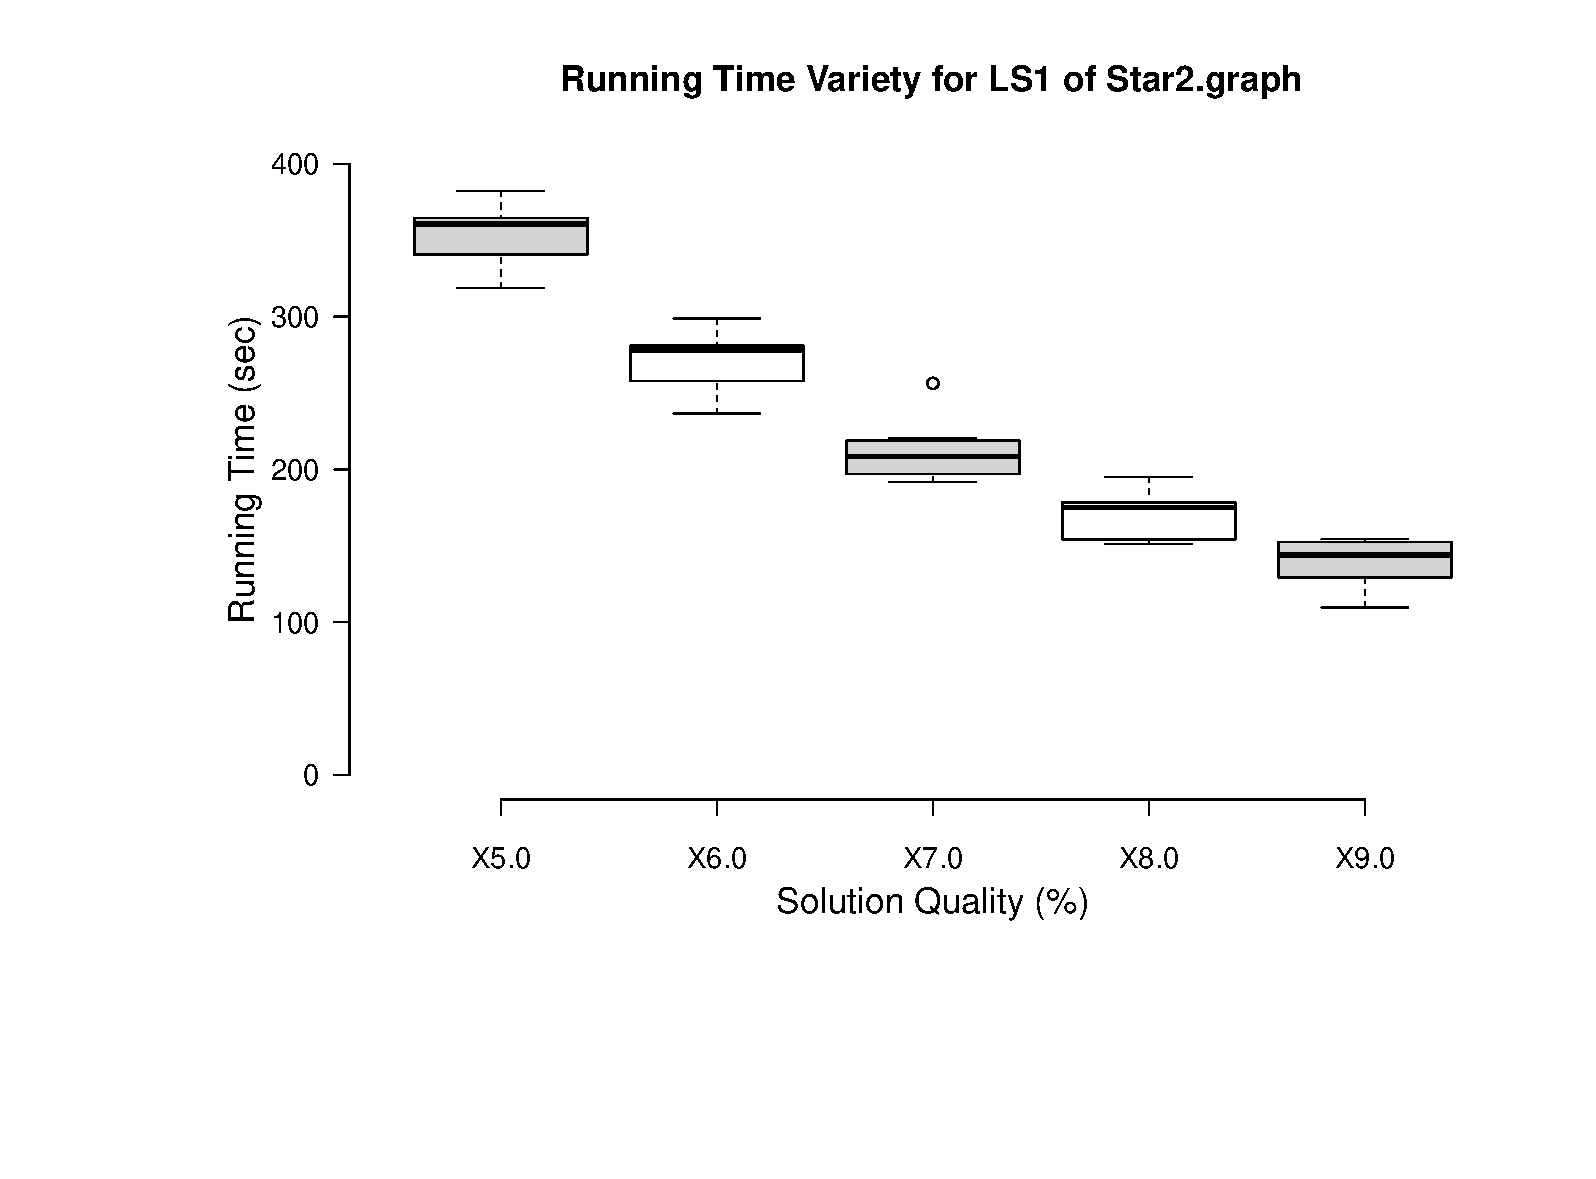
\includegraphics[scale=0.33]{Star2LS1_boxplot.eps}
\end{figure}

\begin{figure}
\centering
\caption{Power QRTD for Local Search 1}
\includegraphics[scale=0.4]{PowerLS1_qrtd_graph.png}
\end{figure}

\begin{figure}
\centering
\caption{Power SQD for Local Search 1}
\includegraphics[scale=0.4]{PowerLS1_sqd_graph.png}
\end{figure}

\begin{figure}
\centering
\caption{Power Box Plot for Local Search 1}
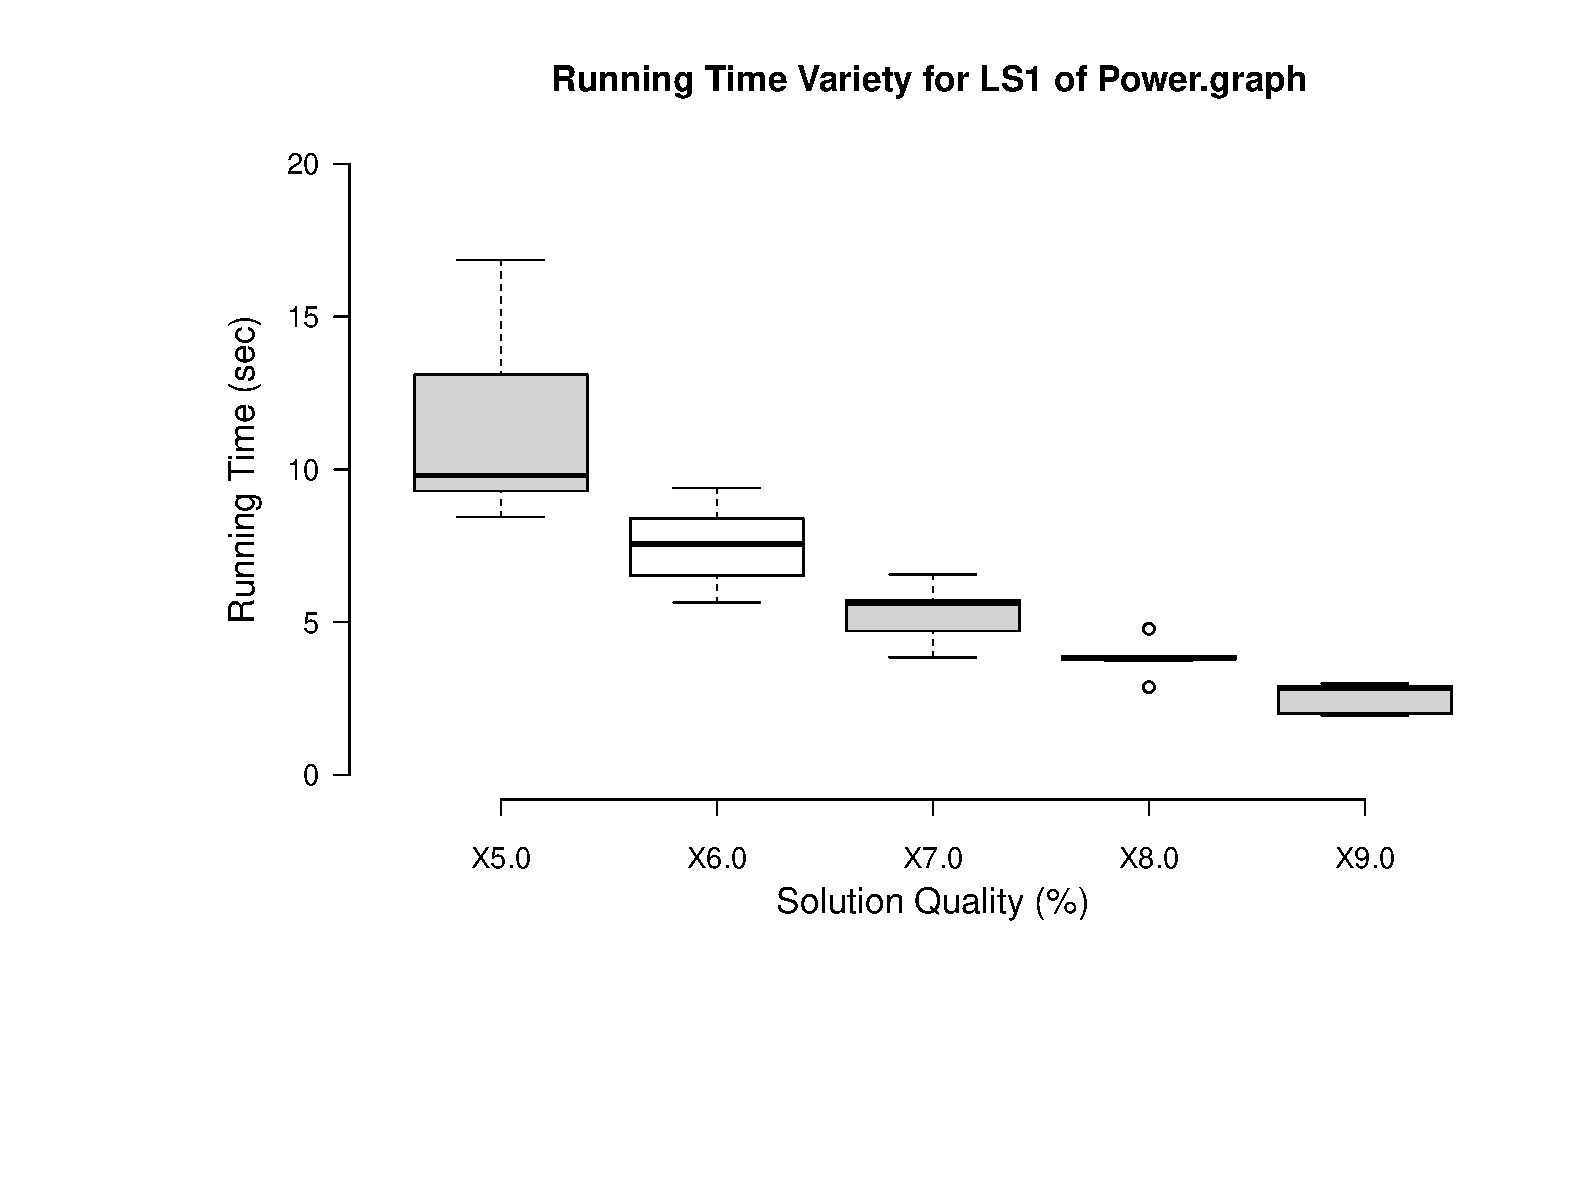
\includegraphics[scale=0.33]{PowerLS1_boxplot.eps}
\end{figure}

\begin{figure}
\centering
\caption{Star 2 QRTD for Local Search 2}
\includegraphics[scale=0.4]{Star2LS2_qrtd_graph.png}
\end{figure}

\begin{figure}
\centering
\caption{Star 2 SQD for Local Search 2}
\includegraphics[scale=0.4]{Star2LS2_sqd_graph.png}
\end{figure}

\begin{figure}
\centering
\caption{Star 2 Box Plot for Local Search 2}
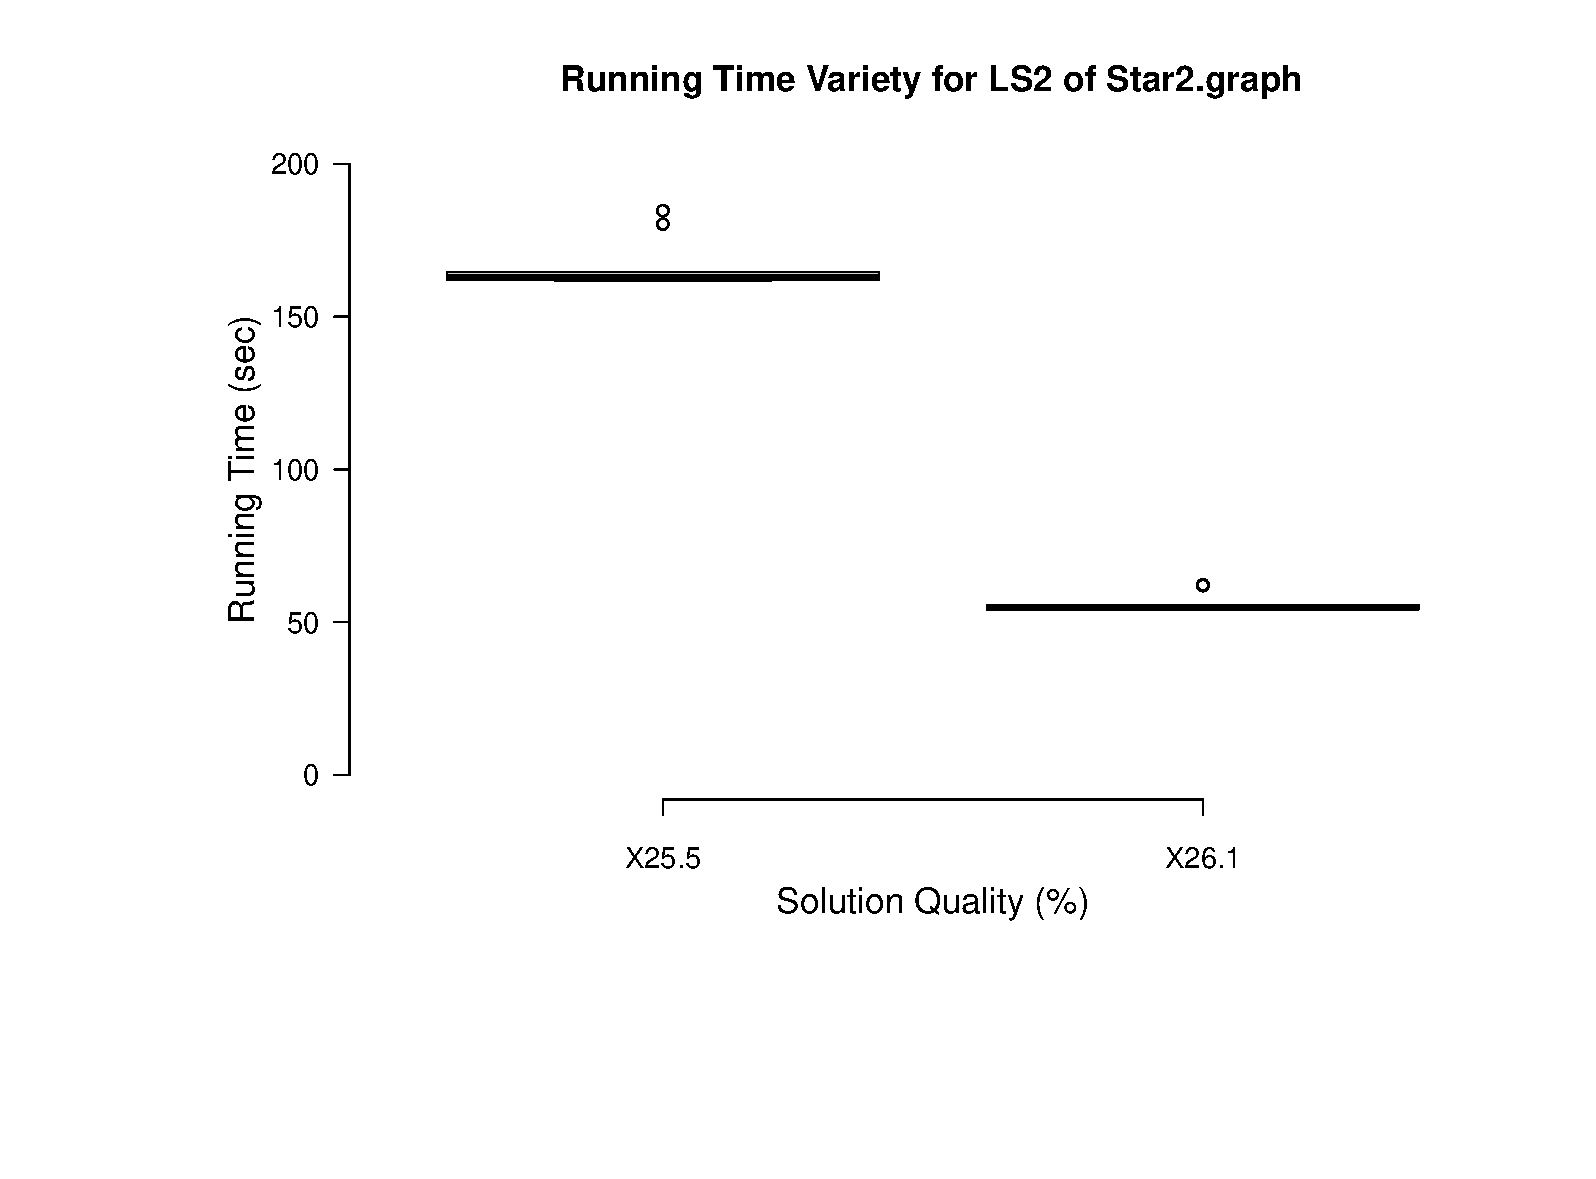
\includegraphics[scale=0.33]{Star2LS2_boxplot.eps}
\end{figure}

\begin{figure}
\centering
\caption{Power QRTD for Local Search 2}
\includegraphics[scale=0.4]{PowerLS2_qrtd_graph.png}
\end{figure}

\begin{figure}
\centering
\caption{Power SQD for Local Search 2}
\includegraphics[scale=0.4]{PowerLS2_sqd_graph.png}
\end{figure}

\begin{figure}
\centering
\caption{Power Box Plot for Local Search 2}
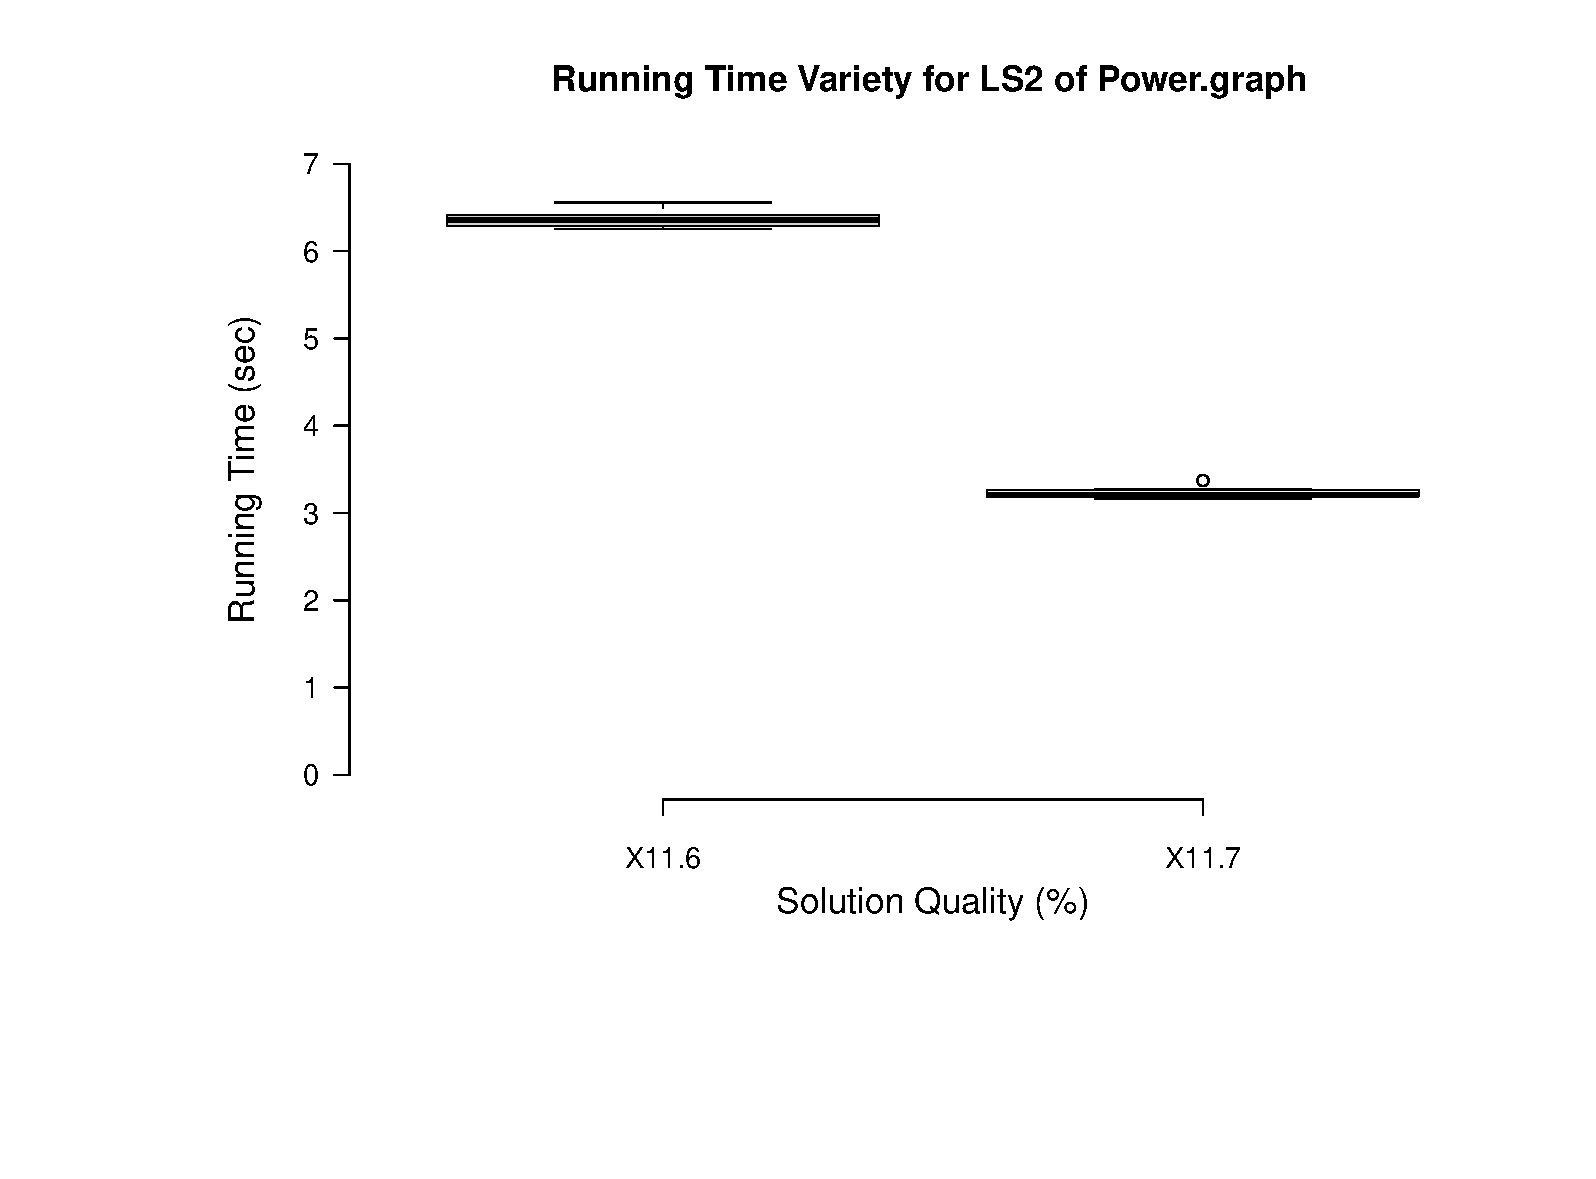
\includegraphics[scale=0.33]{PowerLS2_boxplot.eps}
\end{figure}




\end{document}
